\chapter{KAJIAN PUSTAKA}

\section{Penelitian Terdahulu}

\begin{longtable}{|p{0.5cm}|p{4cm}|p{5cm}|}
	\caption{Tinjauan Penelitian Terdahulu} \\
	\hline
	\textbf{No} & \textbf{Profil Pustaka} & \textbf{Metode dan Temuan Utama} \\ \hline
	\endfirsthead
	\hline
	\textbf{No} & \textbf{Profil Pustaka} & \textbf{Metode dan Temuan Utama} \\ \hline
	\endhead
	\hline
	\multicolumn{3}{r}{\textit{Bersambung ke halaman berikutnya}} \\
	\endfoot
	\hline
	\endlastfoot
	
	1 & 
	\textbf{Judul:} \textit{AcademicRAG: Knowledge Graph Enhanced Retrieval-Augmented Generation for Academic Resource Discovery} \newline
	\textbf{Penulis:} Qiang Sun, dkk. (2024) \cite{sun2024docs2kg} &
	\textbf{Metode:} Mengembangkan kerangka kerja \textit{dual-path} (\textit{Image Converter} dan \textit{Markdown Converter}) untuk mengolah sumber data heterogen (PDF, HTML, Excel, dll.) menjadi satu KG terpadu. \newline
	\textbf{Temuan:} Efektif dalam mengintegrasikan "danau dokumen" yang beragam, memungkinkan kueri lintas format dan menyediakan fondasi untuk aplikasi \textit{knowledge-grounded RAG}. \\
	\hline 
	
	2 & 
	\textbf{Judul:} \textit{CourseKG: An Educational Knowledge Graph Based on Course Information for Precision Teaching} \newline
	\textbf{Penulis:} Ying Li, dkk. (2024) \cite{coursekg} &
	\textbf{Metode:} Menggunakan model \textbf{BERT-BiGRU-MHSA-CRF} untuk \textit{Named Entity Recognition} (NER) pada domain pendidikan dan ekstraksi relasi berbasis \textit{cosine similarity}. \newline
	\textbf{Temuan:} Berhasil membangun KG kurikulum yang komprehensif dari materi perkuliahan, mendukung pemetaan prasyarat dan jalur belajar personal. \\
	\hline
	
	3 & 
	\textbf{Judul:} \textit{Knowledge Graph Generation and Application for Unstructured Data...} \newline
	\textbf{Penulis:} Sushmi T. Sukumar, dkk. (2024) \cite{thushara2024} &
	\textbf{Metode:} Membangun dan mengevaluasi \textit{pipeline} \textit{end-to-end} untuk konstruksi KG, dengan membandingkan performa model ekstraksi relasi OpenNRE vs. REBEL. \newline
	\textbf{Temuan:} Model REBEL (akurasi 87\%) terbukti jauh lebih unggul daripada OpenNRE (61.4\%). Menegaskan efektivitas pendekatan berbasis LLM generatif untuk tugas ekstraksi. \\
	\hline
	
	4 & 
	\textbf{Judul:} \textit{Automatic Construction of Educational Knowledge Graphs...} \newline
	\textbf{Penulis:} Qurat Ul Ain, dkk. (2023) \cite{Ain2023AutomaticCO} &
	\textbf{Metode:} Mengusulkan \textit{pipeline} tanpa supervisi untuk EduKG dengan strategi \textit{keyphrase extraction} sebelum \textit{entity linking} untuk efisiensi, serta pembobotan konsep berbasis SBERT. \newline
	\textbf{Temuan:} Strategi "ekstrak frasa kunci dulu, baru anotasi" terbukti memangkas beban komputasi. Penggunaan SBERT lebih unggul dari TF-IDF untuk pembobotan semantik. \\
	\hline
	
	5 & 
	\textbf{Judul:} \textit{Building a Knowledge Graph for Recommending Experts} \newline
	\textbf{Penulis:} Behzad Rahdari \& Peter Brusilovsky (2019) &
	\textbf{Metode:} Membangun sebuah KG yang memodelkan entitas seperti Peneliti, Publikasi, dan Topik. Menggunakan KG tersebut untuk mengidentifikasi dan merekomendasikan pakar berdasarkan kueri pengguna. \newline
	\textbf{Temuan:} Sistem berbasis KG mampu memberikan rekomendasi pakar yang lebih akurat dan dapat dijelaskan dibandingkan metode tradisional. Relasi antar entitas memungkinkan penemuan pakar yang tidak terdeteksi oleh pencarian kata kunci. \\
	\hline
	
	6 & 
	\textbf{Judul:} \textit{CG-RAG: Research Question Answering by Citation Graph Retrieval-Augmented LLMs} \newline
	\textbf{Penulis:} Yuntong Hu, dkk. (2025) \cite{hu2025cgragresearchquestionanswering} &
	\textbf{Metode:} Mengusulkan kerangka kerja \textbf{Contextualized Graph RAG (CG-RAG)} yang mengintegrasikan sinyal pencarian \textit{sparse} dan \textit{dense} dalam struktur graf. Kerangka ini mencakup representasi graf kutipan kontekstual dan metode pencarian \textbf{Lexical-Semantic Graph Retrieval (LeSeGR)}. \newline
	\textbf{Temuan:} Kerangka kerja CG-RAG secara signifikan mengungguli metode RAG lainnya dalam akurasi pencarian dan kualitas jawaban pada tolok ukur tanya jawab penelitian, dengan memanfaatkan konteks dari graf kutipan. \\
	\hline

    7 & 
    \textbf{Judul:} \textit{University Research Graph Database For Efficient Multi-Perspective Data Analysis Using Neo4j} \newline
    \textbf{Penulis:} \cite{afandi2020university} &
    \textbf{Metode:} Membangun graph database dengan Neo4j yang punya 12 jenis node dan 15 jenis relasi. Data diambil dari Google Scholar, lalu dibentuk jadi graf untuk analisis aktivitas Tri Dharma dosen. \newline
    \textbf{Temuan:} Graph database jauh lebih cepat dibanding database relasional biasa saat menjawab pertanyaan yang rumit. Sistem ini bisa dipakai universitas untuk melihat performa dosen dan pola kolaborasi penelitian mereka. \\
    \hline
\end{longtable}
		
\section{Kajian Teori}

\subsection{Scientific Research}

Terdapat berbagai jenis \textit{knowledge graph} yang berfokus pada penggunaan untuk mendukung proses ilmiah dan membantu peneliti dalam mengeksplorasi pengetahuan penelitian serta mengidentifikasi materi yang relevan \cite{7458844}. Graph-graph ini umumnya menggambarkan seperti, dokumen (misalnya, artikel penelitian, paten), subjek (misalnya, penulis, organisasi), entitas (misalnya, topik, tugas, teknologi), dan informasi kontekstual lainnya (misalnya, proyek, pendanaan) sedemikian rupa sehingga saling terhubung.

\subsection{Knowledge Graph}

\textit{Knowledge Graph} (KG) atau Graf Pengetahuan merupakan pendekatan terstruktur dalam merepresentasikan pengetahuan yang mengaitkan beragam entitas beserta relasinya dalam sebuah bentuk yang terstruktur. Secara matematis, KG dimodelkan sebagai graf berarah $G = (E, R, T)$, di mana $E$ mewakili sebuah entitas (misalnya individu, konsep, atau peristiwa), $R$ mewakili sebuah relasi seperti "mengajar", "bagian\_dari", atau "berafiliasi\_dengan", dan $T \subseteq E \times R \times E$ merepresentasikan sebuah triplet \cite{Hogan_2021}. Setiap triplet $(h, r, t) \in T$ merangkum satu pengetahuan contohnya entitas kepala (\textit{head}) $h$ terhubung secara relasional dengan entitas ekor (\textit{tail}) $t$ melalui relasi $r$. Sebagai ilustrasi, triplet (Jakarta, IBUKOTA, Indonesia) atau (Prabowo, Presiden, Indonesia) mengabstraksikan relasi yang dalam domain geopolitik. Struktur berbasis graf ini memungkinkan adanya penalaran, penelusuran, dan pengintegrasian sumber data heterogen secara efektif, yang membuat KG menjadi tak tergantikan dalam sistem pemahaman semantik dan dalam pengambil sebuah keputusan.
		
Pembangunan KG melibatkan beberapa tahapan utama. Tahap awal adalah akuisisi pengetahuan melalui ekstraksi dari sumber teks tidak terstruktur menggunakan teknik \textit{Natural Language Processing} (NLP) seperti \textit{Named Entity Recognition} untuk mengidentifikasi berbagai entitas dan \textit{Relation Extraction} untuk menemukan relasi di antara entitas dan mengintegrasikan dengan data terstruktur dari basis-basis pengetahuan yang sudah ada (misal Wikidata \cite{wikidata}) yang bertujuan memperluas cakupan Knowledge. KG yang telah terbentuk dapat diperkaya melalui pendekatan seperti (\textit{link prediction}) atau penalaran berbasis aturan untuk menginferensi fakta baru. Misalnya, KnowEdu yang berfokus di bidang pendidikan menggunakan teknik \textit{neural sequence labeling} dan aturan asosiasi probabilistik untuk mengekstraksi konsep-konsep pedagogis serta hubungan prasyaratnya dari data kurikulum \cite{knowedu}.Saat ini, dengan kemajuan pesat Model Bahasa Besar (LLM) dalam pemahaman semantik dan ekstraksi entitas, berbagai penelitian mulai memanfaatkan LLM untuk mengotomatisasi serta meningkatkan akurasi proses pembangunan KG \cite{edge2025localglobalgraphrag}.
		
telah diterapkan secara luas di berbagai bidang karena kemampuannya dalam merepresentasikan hubungan yang kompleks serta mengintegrasikan berbagai sumber data:  
\begin{daftar}
	\item Mesin Pencarian dan Pengambilan Informasi: Platform komersial seperti KG Google memanfaatkan hubungan antar entitas untuk memperjelas kueri dan menyediakan informasi kontekstual, yang secara signifikan meningkatkan akurasi pencarian dalam pengujian standar.  
	\item Recommendation Systems: KGs mendukung mesin rekomendasi dengan mengidentifikasi keterkaitan antara preferensi pengguna dan konten, sehingga menghasilkan saran yang lebih relevan.
	\item Healthcare: Knowledge Graphs (KGs) mengintegrasikan sejumlah besar data biomedis, yang membantu dalam penemuan obat, penelitian penyakit, dan pengobatan yang dipersonalisasidengan mengungkap relasi tersembunyi antara entitas biologis.
\end{daftar}

Berbagai penerapan terbaru telah mengintegrasikan Knowledge Graph (KG) dengan Large Language Models (LLM) untuk meningkatkan kemampuan penalaran serta kemampuan LLM dalam menghasilkan jawaban. Contohnya, arsitektur DRAGON \cite{yasunaga2022deepbidirectionallanguageknowledgegraph} berhasil mencapai performa terbaik pada benchmark pertanyaan kompleks seperti CSQA dan OBQA, dengan melatih LLM menggunakan data dari KG sehingga memungkinkan LLM memberikan jawaban yang terstruktur terhadap pertanyaan yang kompleks \cite{saha2018complexsequentialquestionanswering, mihaylov2018suitarmorconductelectricity}. Ke depannya, pengembangan KG diperkirakan akan berfokus pada konstruksi berbasis input multimodal dan eksplorasi embedding graf untuk mendukung pengambilan keputusan secara real-time.
		
\subsection{LLM}
		
\subsection{Pemrosesan Bahasa Alami untuk Ekstraksi Pengetahuan}
		
\subsection{Graf Basis Data}

\subsection{Sistem Rekomendasi}
		
\subsection{Retrieval-Augmented Generation (RAG)}

Retrieval-Augmented Generation (RAG) adalah pendekatan kolaboratif yang menggabungkan kemampuan model bahasa besar (LLM) yang telah dilatih sebelumnya, dengan sistem pencarian informasi eksternal untuk meningkatkan kinerja pada tugas-tugas yang membutuhkan pengetahuan mendalam. \cite{lewis2021retrievalaugmentedgenerationknowledgeintensivenlp,gao2024retrievalaugmentedgenerationlargelanguage}. Berbeda dari model bahasa tradisional yang hanya mengandalkan pengetahuan internal dalam parameter model, RAG memungkinkan sistem untuk mencari dan mengambil dokumen terkait dari database luar sebelum menghasilkan jawaban. Pendekatan ini secara efektif mampu mengatasi keterbatasan LLM terkait dengan risiko halusinasi, ppengetahuan yang usang, dan transparansi yang terbatas yang menjadikan RAG sebuah lompatan penting di dunia pemrosesan bahasa alami.

\begin{figure}[!t]
		\centering
		\makebox[\textwidth][c]{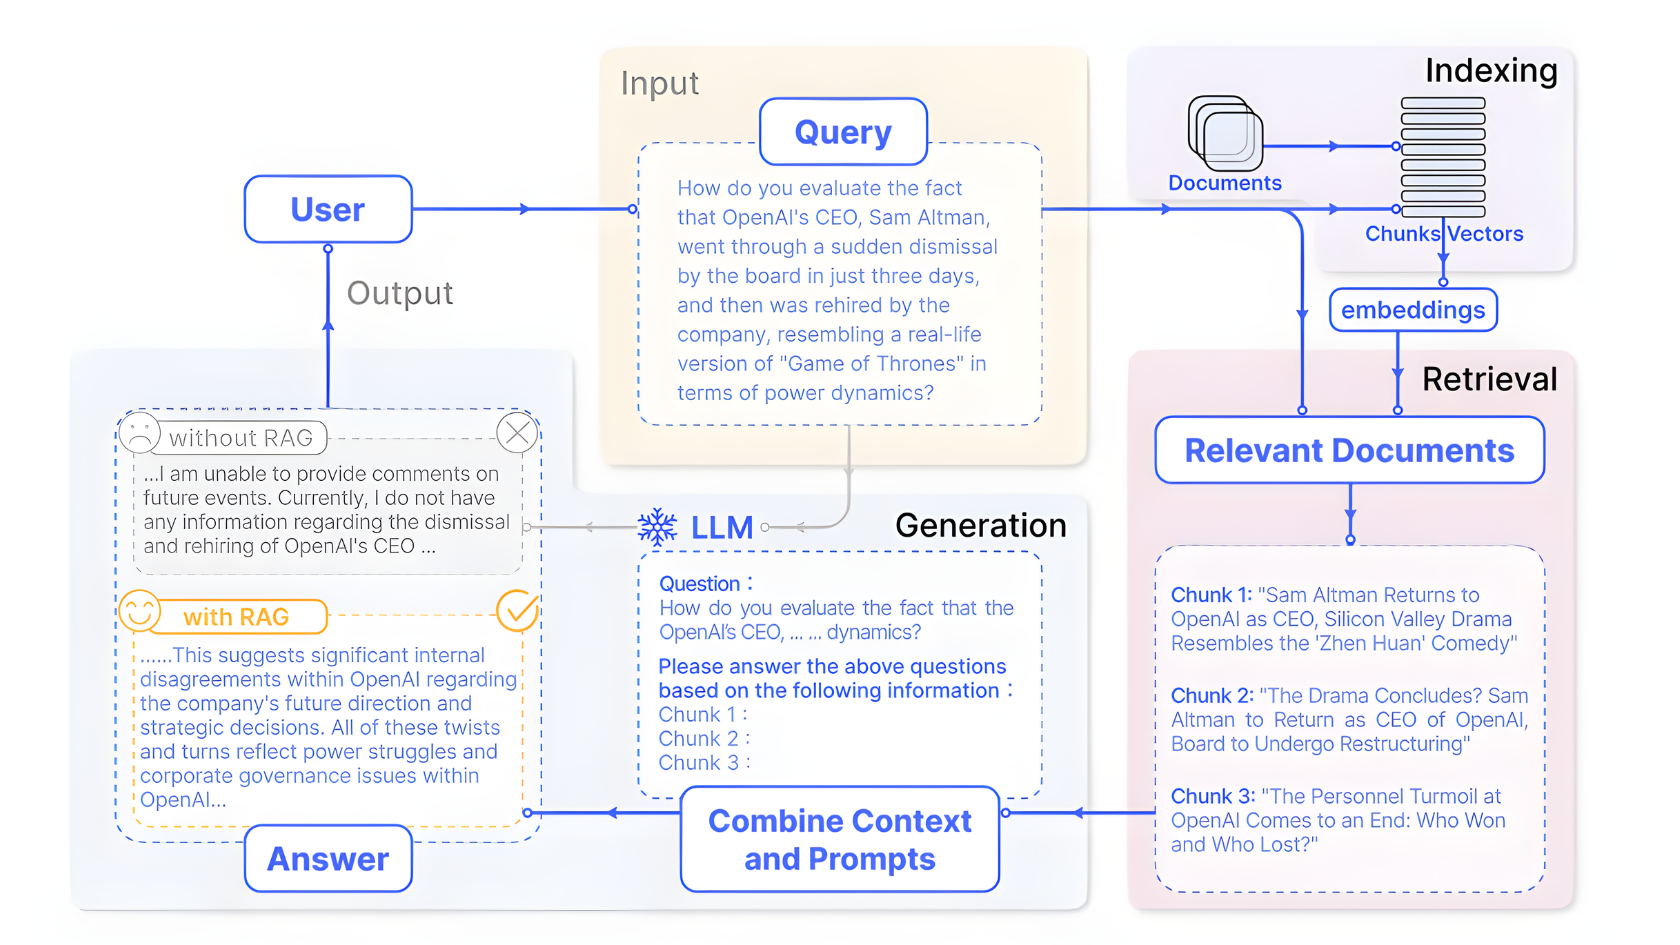
\includegraphics[width=1\textwidth]{Gambar/RAG.png}}
		\caption{Proses Retrieval-Augmented Generation untuk Question Answering \cite{edge2025localglobalgraphrag}}
		\label{fig:rag-process}
\end{figure}

Dengan RAG, LLM bisa secara dinamis memanfaatkan pengetahuan eksternal membuat respons yang dihasilkan menjadi lebih akurat, informatif, dan mutakhir. Proses retrieval mengurangi risiko model "ngarang" jawaban karena jawaban merujuk pada sumber dokumen. Ini membuat RAG sangat unggul dalam domain yang pengetahuannya berkembang cepat, seperti berita, publikasi sains, ataupun regulasi yang berubah secara periodik. Pengguna juga bisa menelusuri dari mana sumber jawaban AI berasal, meningkatkan transparansi dan kepercayaan.
		
Sebagai ilustrasi praktis, misal pengguna ingin mengetahui perkembangan suatu topik berita yang sedang viral beberapa hari terakhir. Model LLM berbasis pre-trained umumnya kurang mampu memberikan informasi terbaru, sehingga respons yang dihasilkan sering kurang relevan dengan konteks aktual. Namun, dengan penerapan skema RAG seperti pada \ref{fig:rag-process}, sistem akan secara otomatis mengambil dan mengintegrasikan dokumen berita terkini sebagai referensi utama, sehingga jawaban yang dihasilkan lebih faktual dan sesuai kebutuhan pengguna.
		
Seiring dengan meningkatnya kebutuhan akan informasi yang akurat dan terkini, RAG telah diintegrasikan dan diadopsi di berbagai bidang aplikasi dalam ekosistem teknologi modern:
\begin{itemize}
	\item \textbf{Open-Domain Question Answering:} RAG terbukti meningkatkan performa QA tanya jawab terbuka karena mampu mengambil referensi dari Wikipedia atau dataset yang relevan, dan secara konsisten melampaui model ekstraktif berbasis machine reading comprehension pada berbagai benchmark seperti pada Natural Questions dan TriviaQA.
	\item \textbf{Aplikasi Legal dan Medis:} Di domain hukum serta kesehatan, RAG digunakan untuk penelusuran dokumen kasus hukum terbaru atau artikel ilmiah medis guna memberi landasan keputusan berbasis data mutakhir dan referensi valid.
	\item \textbf{Chatbot dan Virtual Assistant:} Integrasi RAG pada sistem percakapan seperti ChatGPT memungkinkan respons lebih akurat karena mampu mengambil data keuangan, dokumentasi teknis, ataupun berita terkini secara real-time.
\end{itemize}
\subsection{Graph Based RAG}
\textit{Graph-RAG} adalah sebuah evolusi dari arsitektur RAG yang dirancang untuk meningkatkan mekanisme pengambilan informasi dengan memanfaatkan sumber pengetahuan terstruktur, seperti \textit{Knowledge Graph} (KG) atau basis data relasional \cite{peng2024graphretrievalaugmentedgenerationsurvey}. Berbeda dengan RAG konvensional yang umumnya mengambil potongan teks tidak terstruktur, Graph-RAG secara spesifik mengambil elemen-elemen graf yang relevan—seperti entitas, relasi, atau bahkan seluruh subgraf—untuk memperkaya konteks yang diberikan kepada Model Bahasa Besar (LLM).

Pendekatan ini menghasilkan beberapa keunggulan signifikan seperti, penalaran yang lebih presisi, akurasi faktual yang lebih tinggi, serta \textbf{interpretasi dan transparansi} yang lebih baik, karena respons yang dihasilkan dapat dilacak kembali ke entitas dan relasi spesifik di dalam graf. Hal ini menjadikan Graph-RAG sangat ideal untuk aplikasi yang menuntut konsistensi logika dan pemahaman mendalam terhadap hubungan antar-entitas, seperti pada sistem rekomendasi akademik yang akan dikembangkan dalam penelitian ini.
		
\subsubsection{Rumus}
	Rumus umum persamaan pythagoras diberikan oleh persamaan~\ref{fig:rag-process} berikut ini
\begin{equation}
	a^2 + b^2 = c^2 \label{eq:pythagoras}
\end{equation}
		
Model penyebaran penyakit diberikan oleh sistem persamaan diferensial sebagai berikut:
	\begin{align}
		\frac{dS}{dt} &= \beta S I\\
		\nonumber \frac{dI}{dt} &= -\beta S I
	\end{align}
		
	\begin{equation}
		\begin{aligned}
			\frac{dS}{dt} &= \beta S I\\
			\frac{dI}{dt} &= -\beta S I
		\end{aligned}
	\end{equation}
		
	\begin{equation}
		I = \int_0^{\infty} e^{at}~{dt}
	\end{equation}
		
Matriks Identitas $3 \times 3$ diberikan oleh:
	\begin{equation}
		I = \begin{bmatrix}
			1 & 0 & \cdots & 0\\
			0 & 1 & \cdots & \vdots\\
			\cdots & \cdots & \ddots &\vdots\\
			0 & 0 & \cdots & 1
		\end{bmatrix}
	\end{equation}
		
	\begin{theorem}[Teorema Keterbagian]
		Diberikan bilangan bulat  $a$, $b$, dan $c$ dengan $a \neq 0$ sehingga berlaku sifat-sifat berikut ini.
	\end{theorem}
		
	\begin{theorem}[Teorema Keterbagian]
		Diberikan bilangan bulat  $a$, $b$, dan $c$ dengan $a \neq 0$ sehingga berlaku sifat-sifat berikut ini.
	\end{theorem}
		
	\begin{proof}
		Berdasarkan $\cdots$
	\end{proof}
		
	\begin{definition}
		Diberikan bilangan bulat $a$ dan $b$ dengan $a \neq 0$. Jika $b$ merupakan kelipatan dari $a$, maka kita katakan bahwa  $a$ habis membagi $b$ atau dinotasikan $a|b$
	\end{definition}
		
	\begin{example}
		Diberikan bilangan bulat $a$ dan $b$ dengan $a \neq 0$. Jika $b$ merupakan kelipatan dari $a$, maka kita katakan bahwa  $a$ habis membagi $b$ atau dinotasikan $a|b$
	\end{example}
		
	\begin{theorem}
		Diberikan bilangan bulat  $a$, $b$, dan $c$ dengan $a \neq 0$ sehingga berlaku sifat-sifat berikut ini.
	\end{theorem}

\section{test}

		
\section{Hasil Penelitian yang Relevan}
	Hasil Penelitian yang relevan berfungsi memperkuat posisi penelitian yang dilakukan saat ini dengan melihat hasil-hasil penelitian yang sudah dilakukan. Hasil penelitian yang relevan juga digunakan sebagai dasar peneliti menyusun kerangka berpikir. Hasil penelitian yang relevan disajikan secara narasi dengan menganalisis hasil penelitian yang satu dengan hasil penelitian yang lain.
		
\section{Kerangka Berpikir}
	Kerangka Berpikir berisikan gambaran logis dan rasional tentang bagaimana variable-variabel penelitian dapat saling berhubungan (korelasi). Kerangka berpikir akan mengarahkan peneliti kepada perumusan hipotesis. Penelitianyang tidak membuktikan hipotesis seperti penelitian dengan pendekatan kualitatif, tidak perlu menuliskan kerangka berpikir.
		
\section{Pertanyaan Penelitian dan/atau Hipotesis (jika ada)}
	Pertanyaan penelitian merupakan penegasan dari rumusan masalah yang akan dicari jawabannya melalui penelitian. Hipotesis merupakan jawaban sementara terhadap rumusan masalah yang dinyatakan dengan kalimat pernyataan. Untuk penelitian yang tidak membuktikan hipotesis cukup menuliskan pertanyaan penelitian. Hipotesis atau pertanyaan penelitian harus selaras dan merupakan jabaran dari rumusan masalah.